\section{Bilder}

%\begin{figure}
%    \centering
%    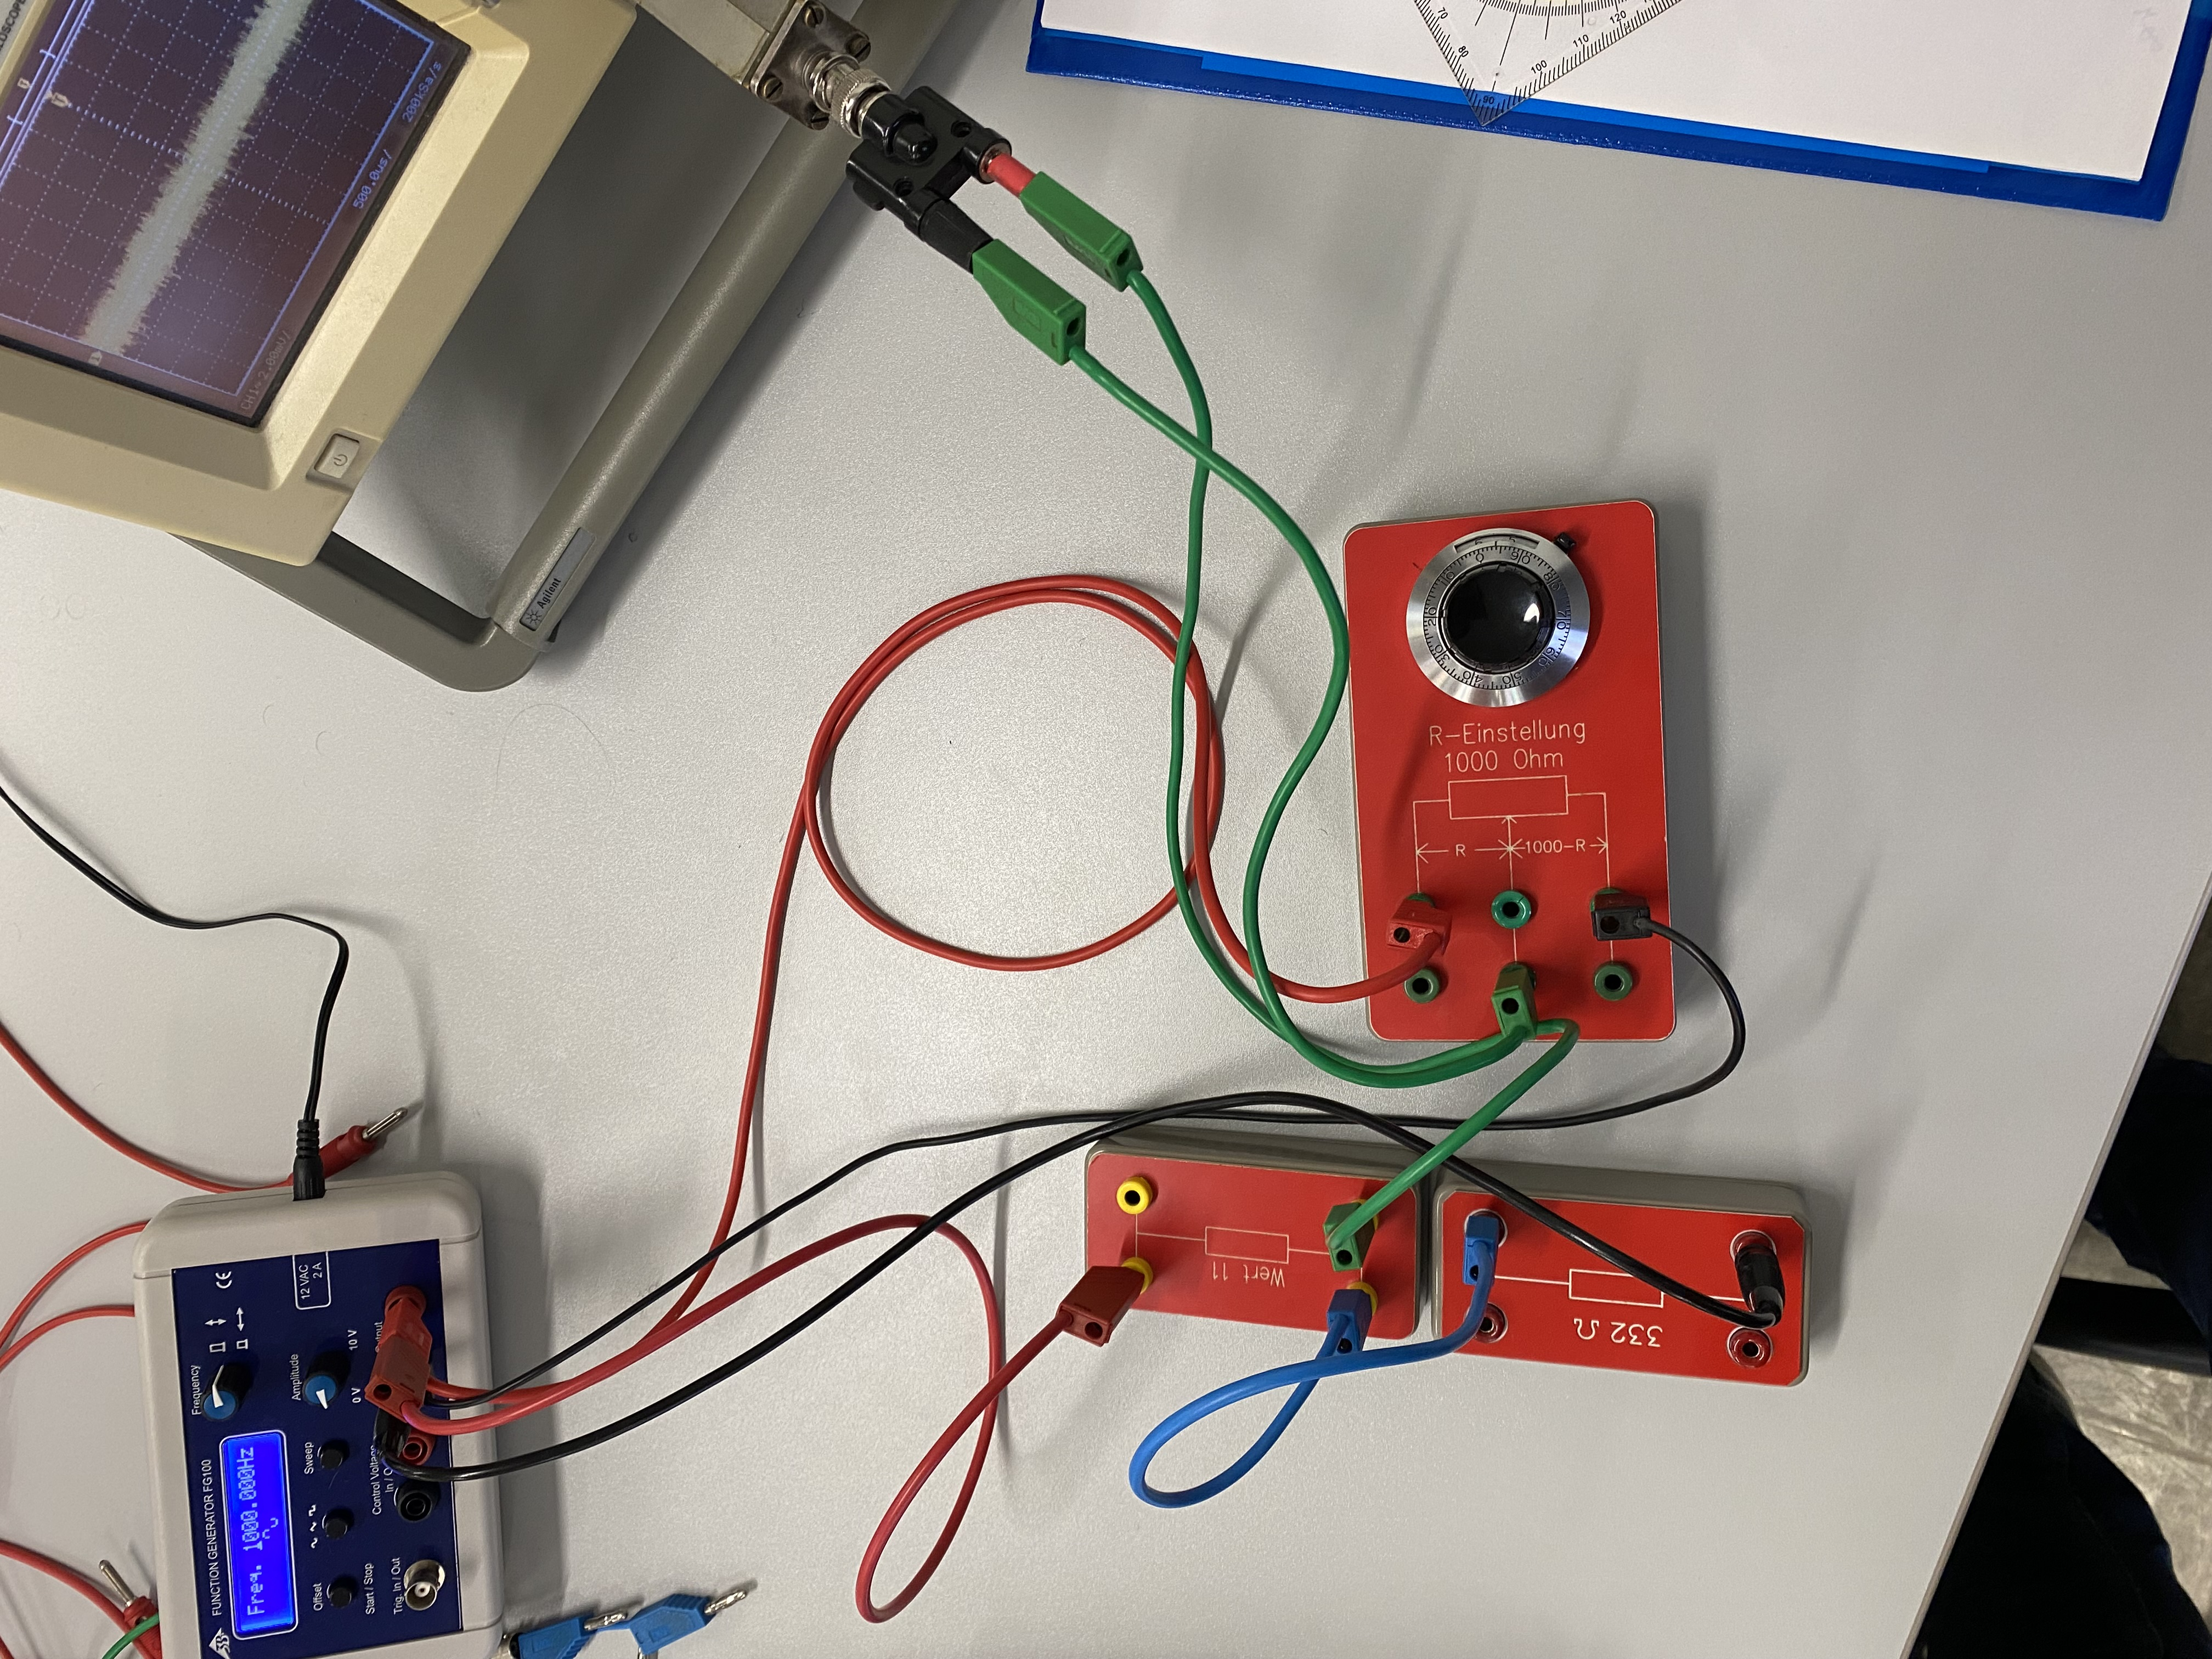
\includegraphics[scale=0.1]{Bilder/wheat.jpg}
%    \caption{Die Wheatstonesche Brückenschaltung}
%    \label{fig:wheat}
%  \end{figure}
%  \begin{figure}
%    \centering
%    \includegraphics[scale=0.1]{Bilder/kapazität.jpg}
%    \caption{Die kapazitive Brückenschaltung}
%    \label{fig:kapaz}
%  \end{figure}
%  \begin{figure}
%    \centering
%    \includegraphics[scale=0.1]{Bilder/induktivität.jpg}
%    \caption{Die induktive Brückenschaltung}
%    \label{fig:induk}
%  \end{figure}
%  \begin{figure}
%    \centering
%    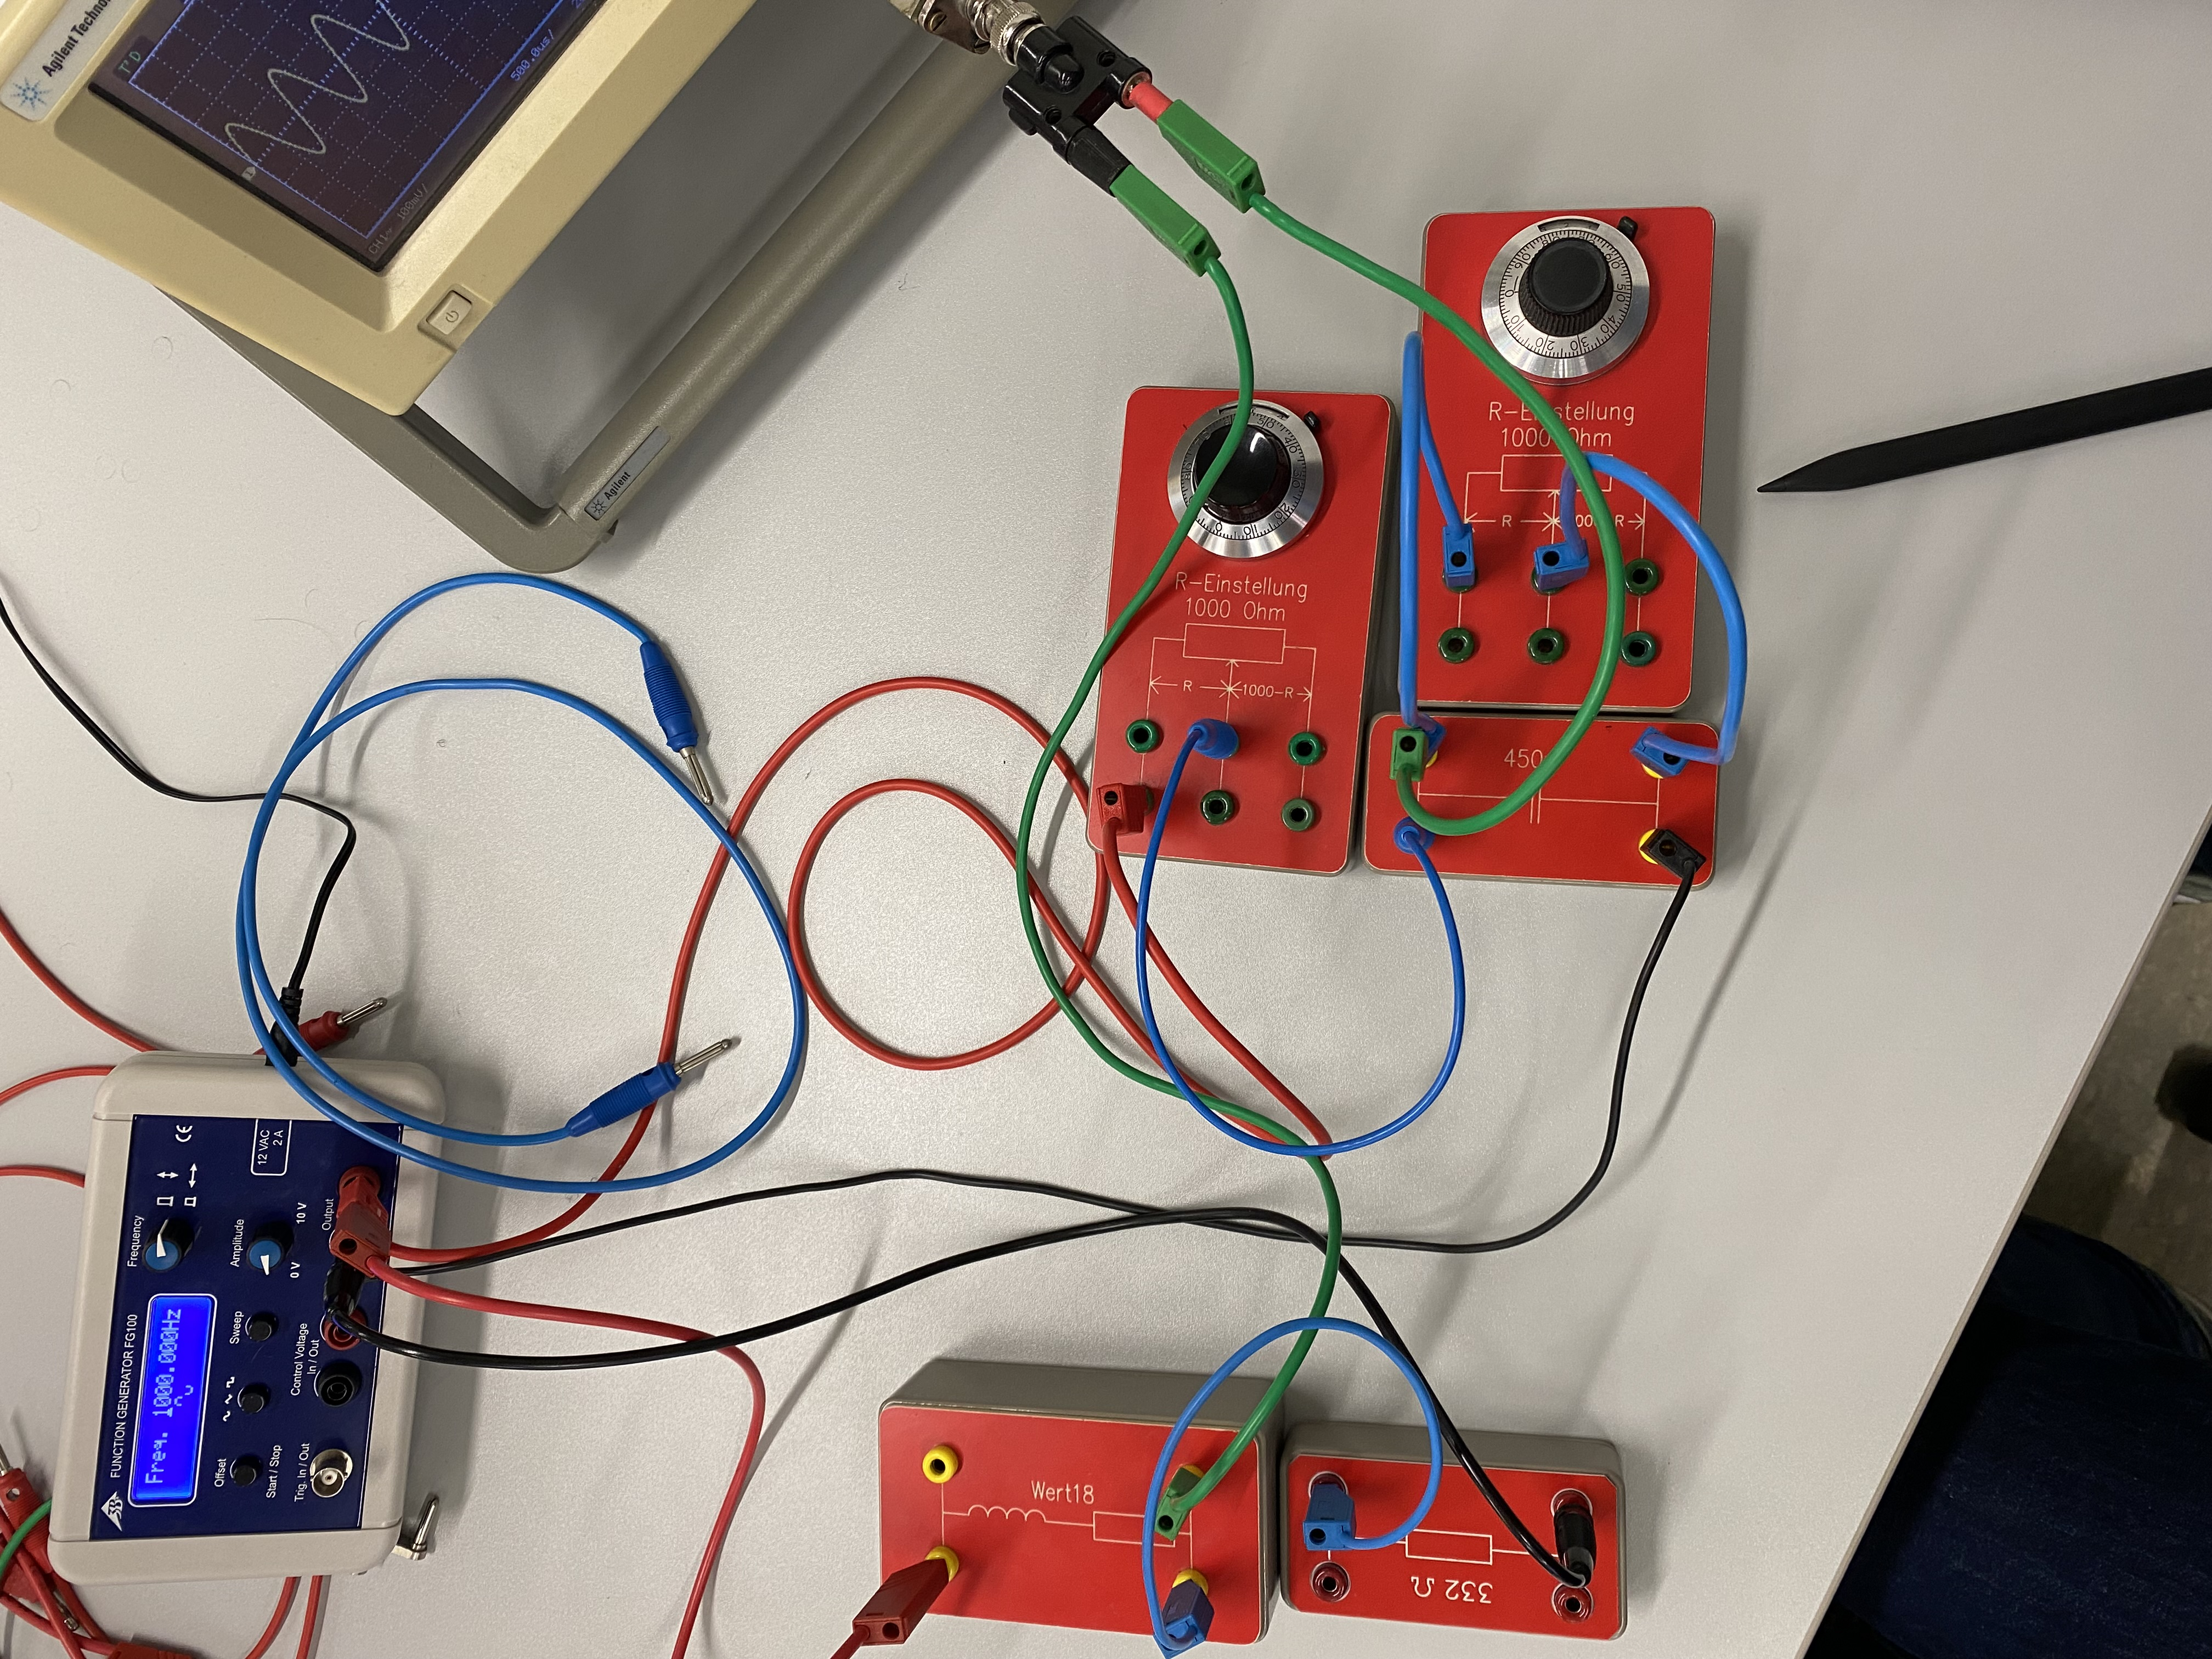
\includegraphics[scale=0.1]{Bilder/maxwellsche.jpg}
%    \caption{Die Maxwellsche Brückenschaltung}
%    \label{fig:max}
%  \end{figure}
%  \begin{figure}
%    \centering
%    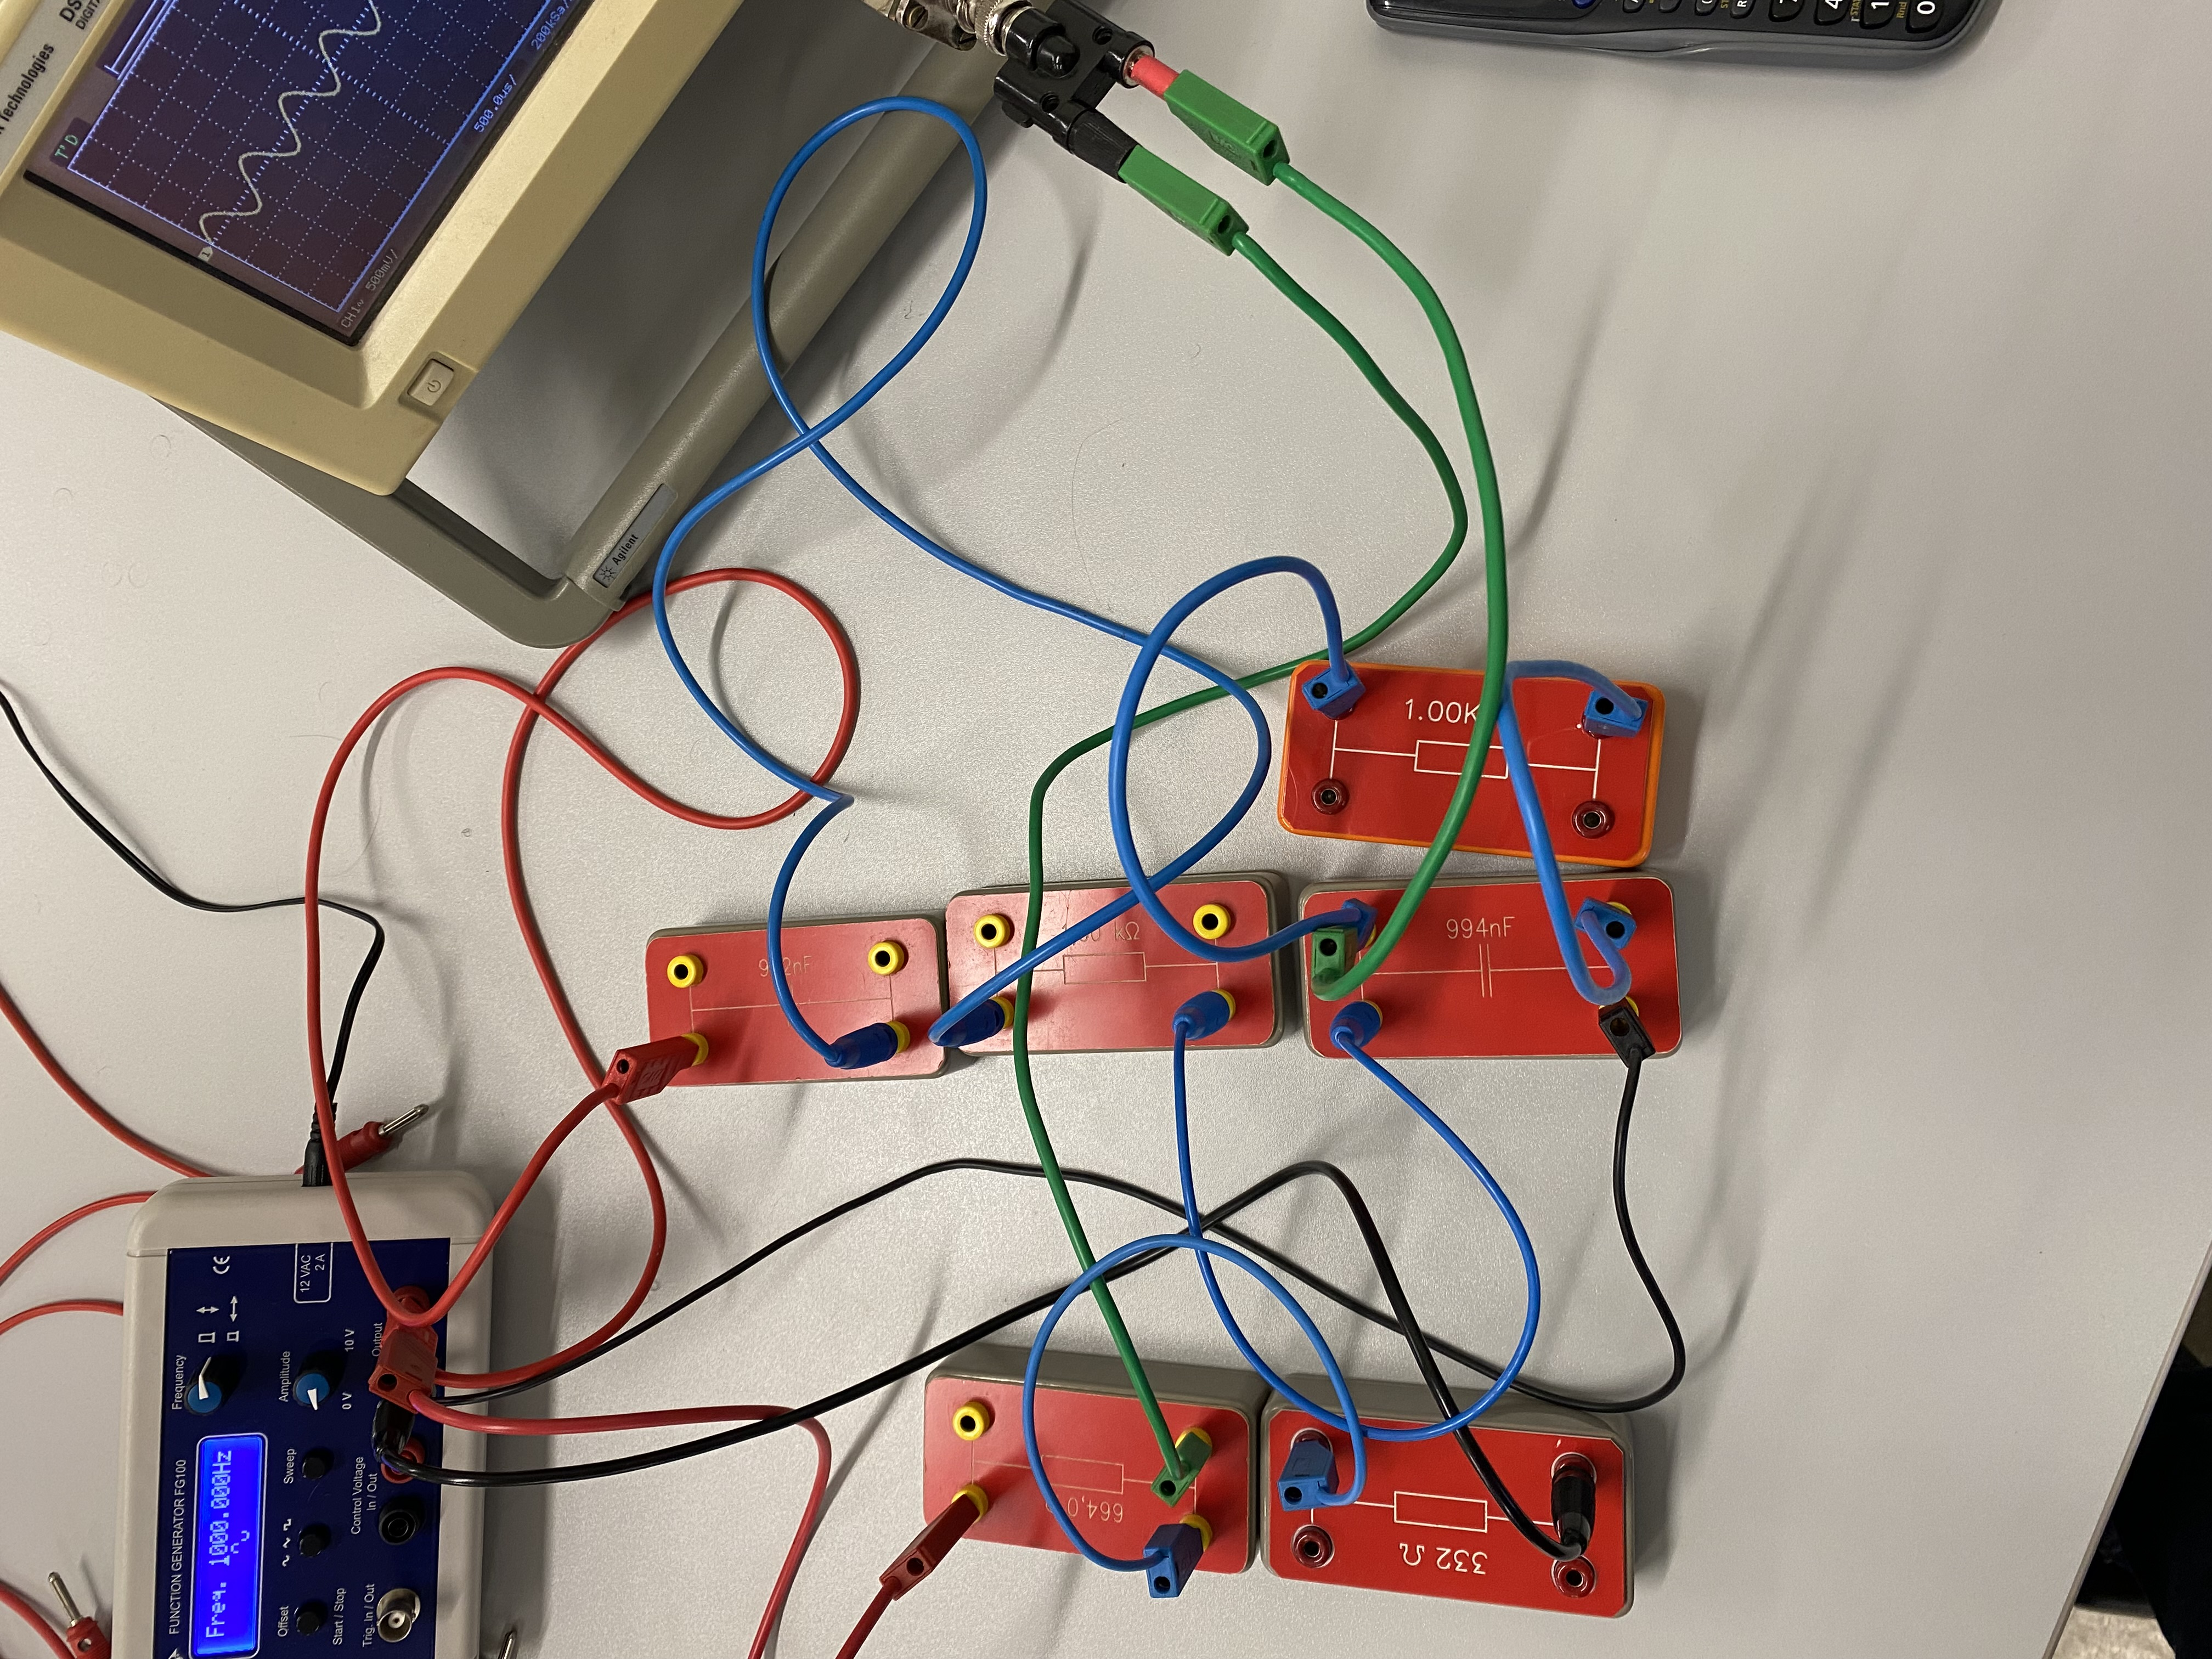
\includegraphics[scale=0.1]{Bilder/wien.jpg}
%    \caption{Die Wien-Robinson Brückenschaltung}
%    \label{fig:wheat}
%  \end{figure}
  %\begin{figure}
  %  \centering
  %  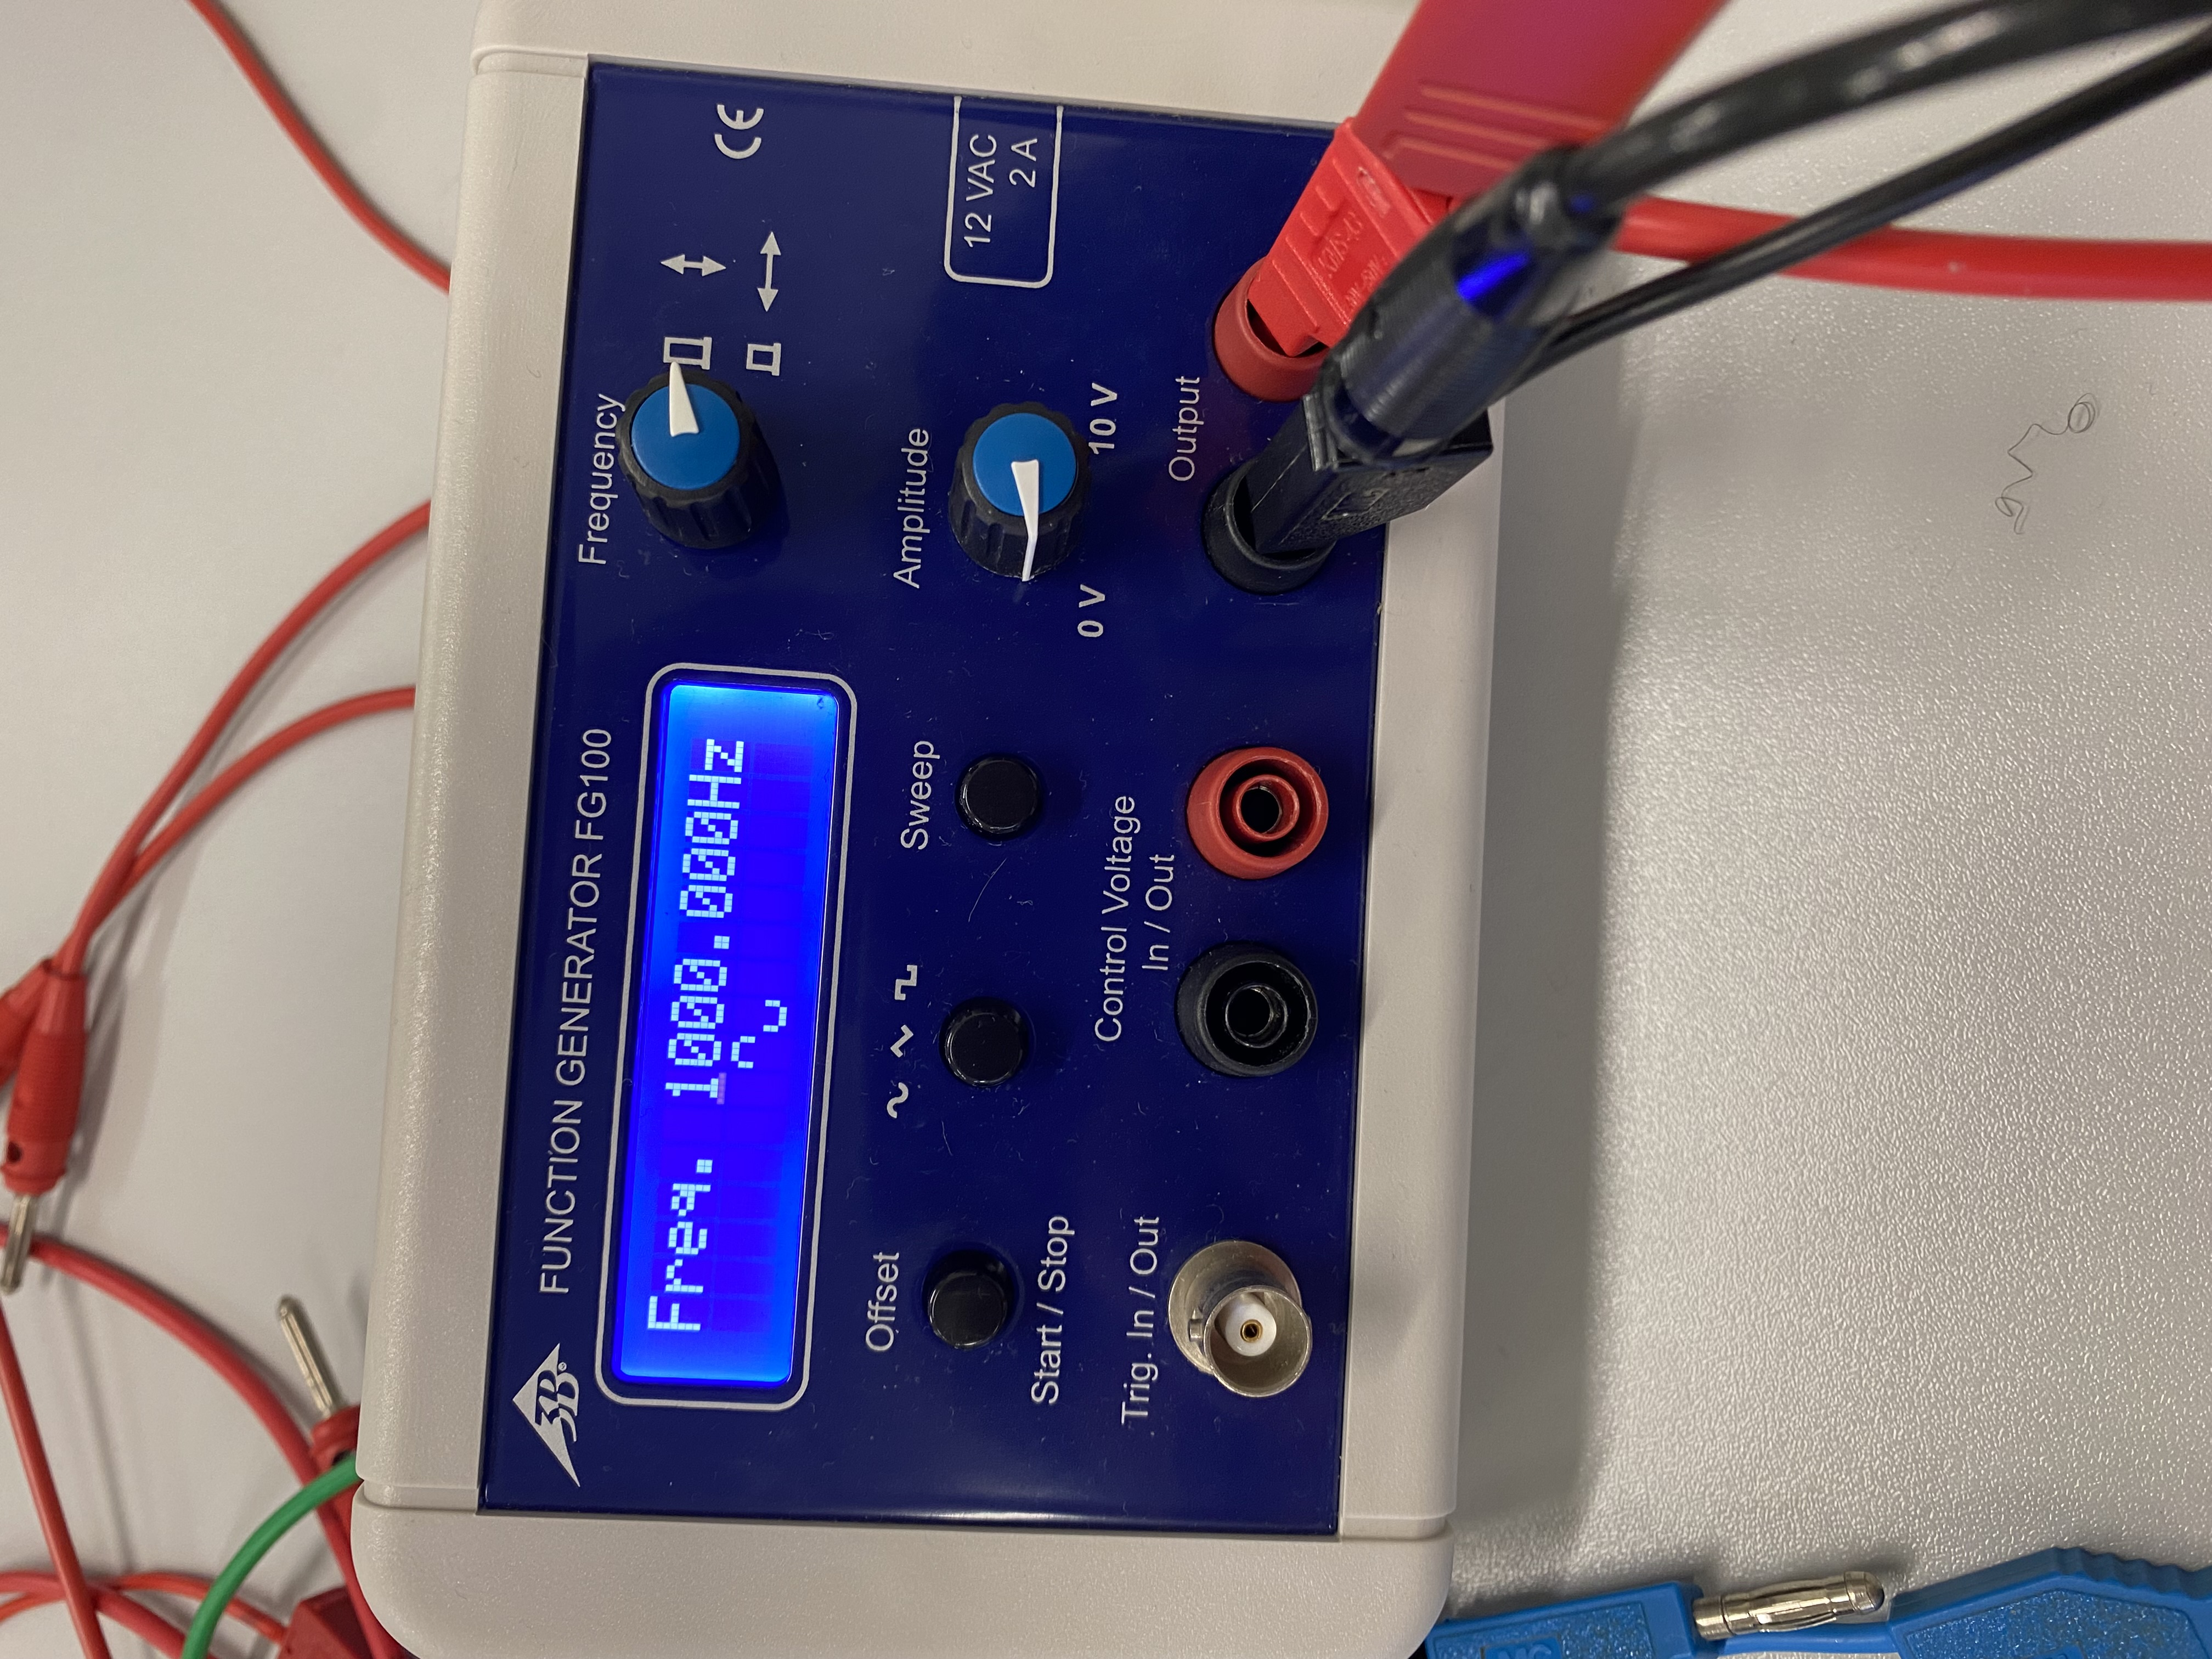
\includegraphics[scale=0.1, angle=270]{Bilder/spannungsquelle.jpg}
  %  \caption{Die Wechselspannungsquelle}
  %  \label{fig:spann}
  %\end{figure}
  \begin{figure}
    \centering
    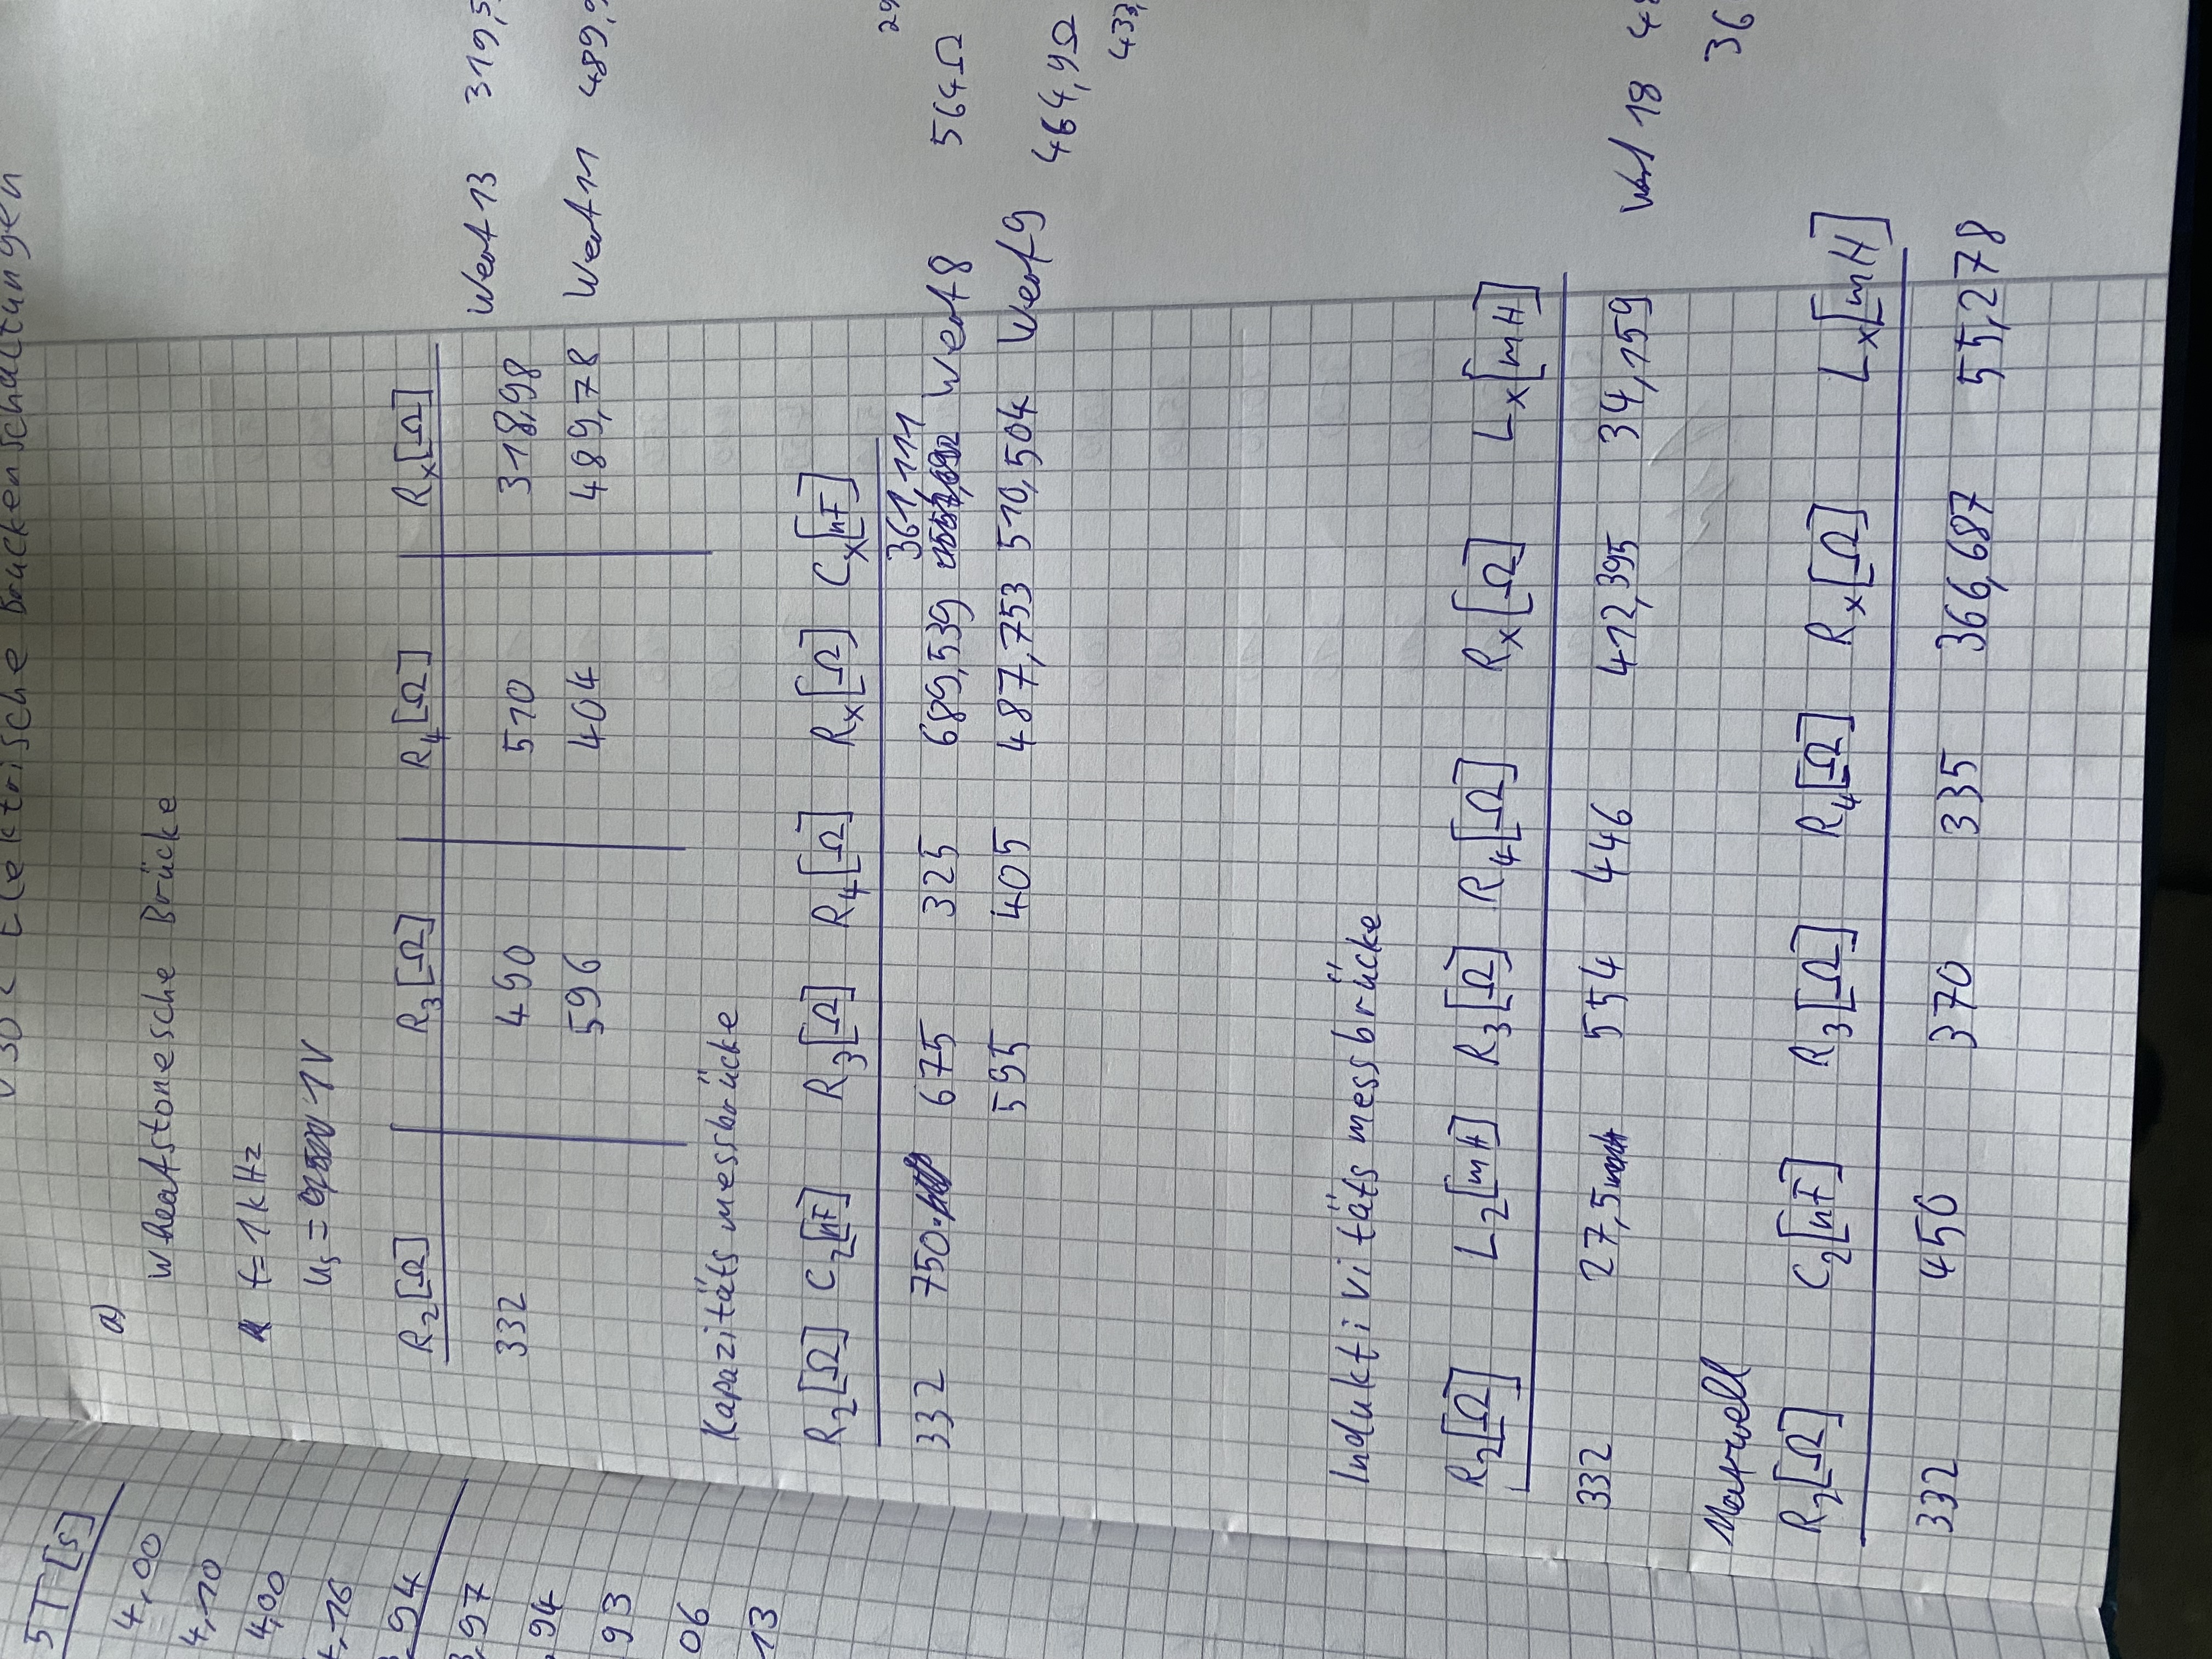
\includegraphics[scale=0.1, angle=270]{Bilder/mess1.jpg}
    
    \label{fig:mess1}
  \end{figure}
  \begin{figure}
    \centering
    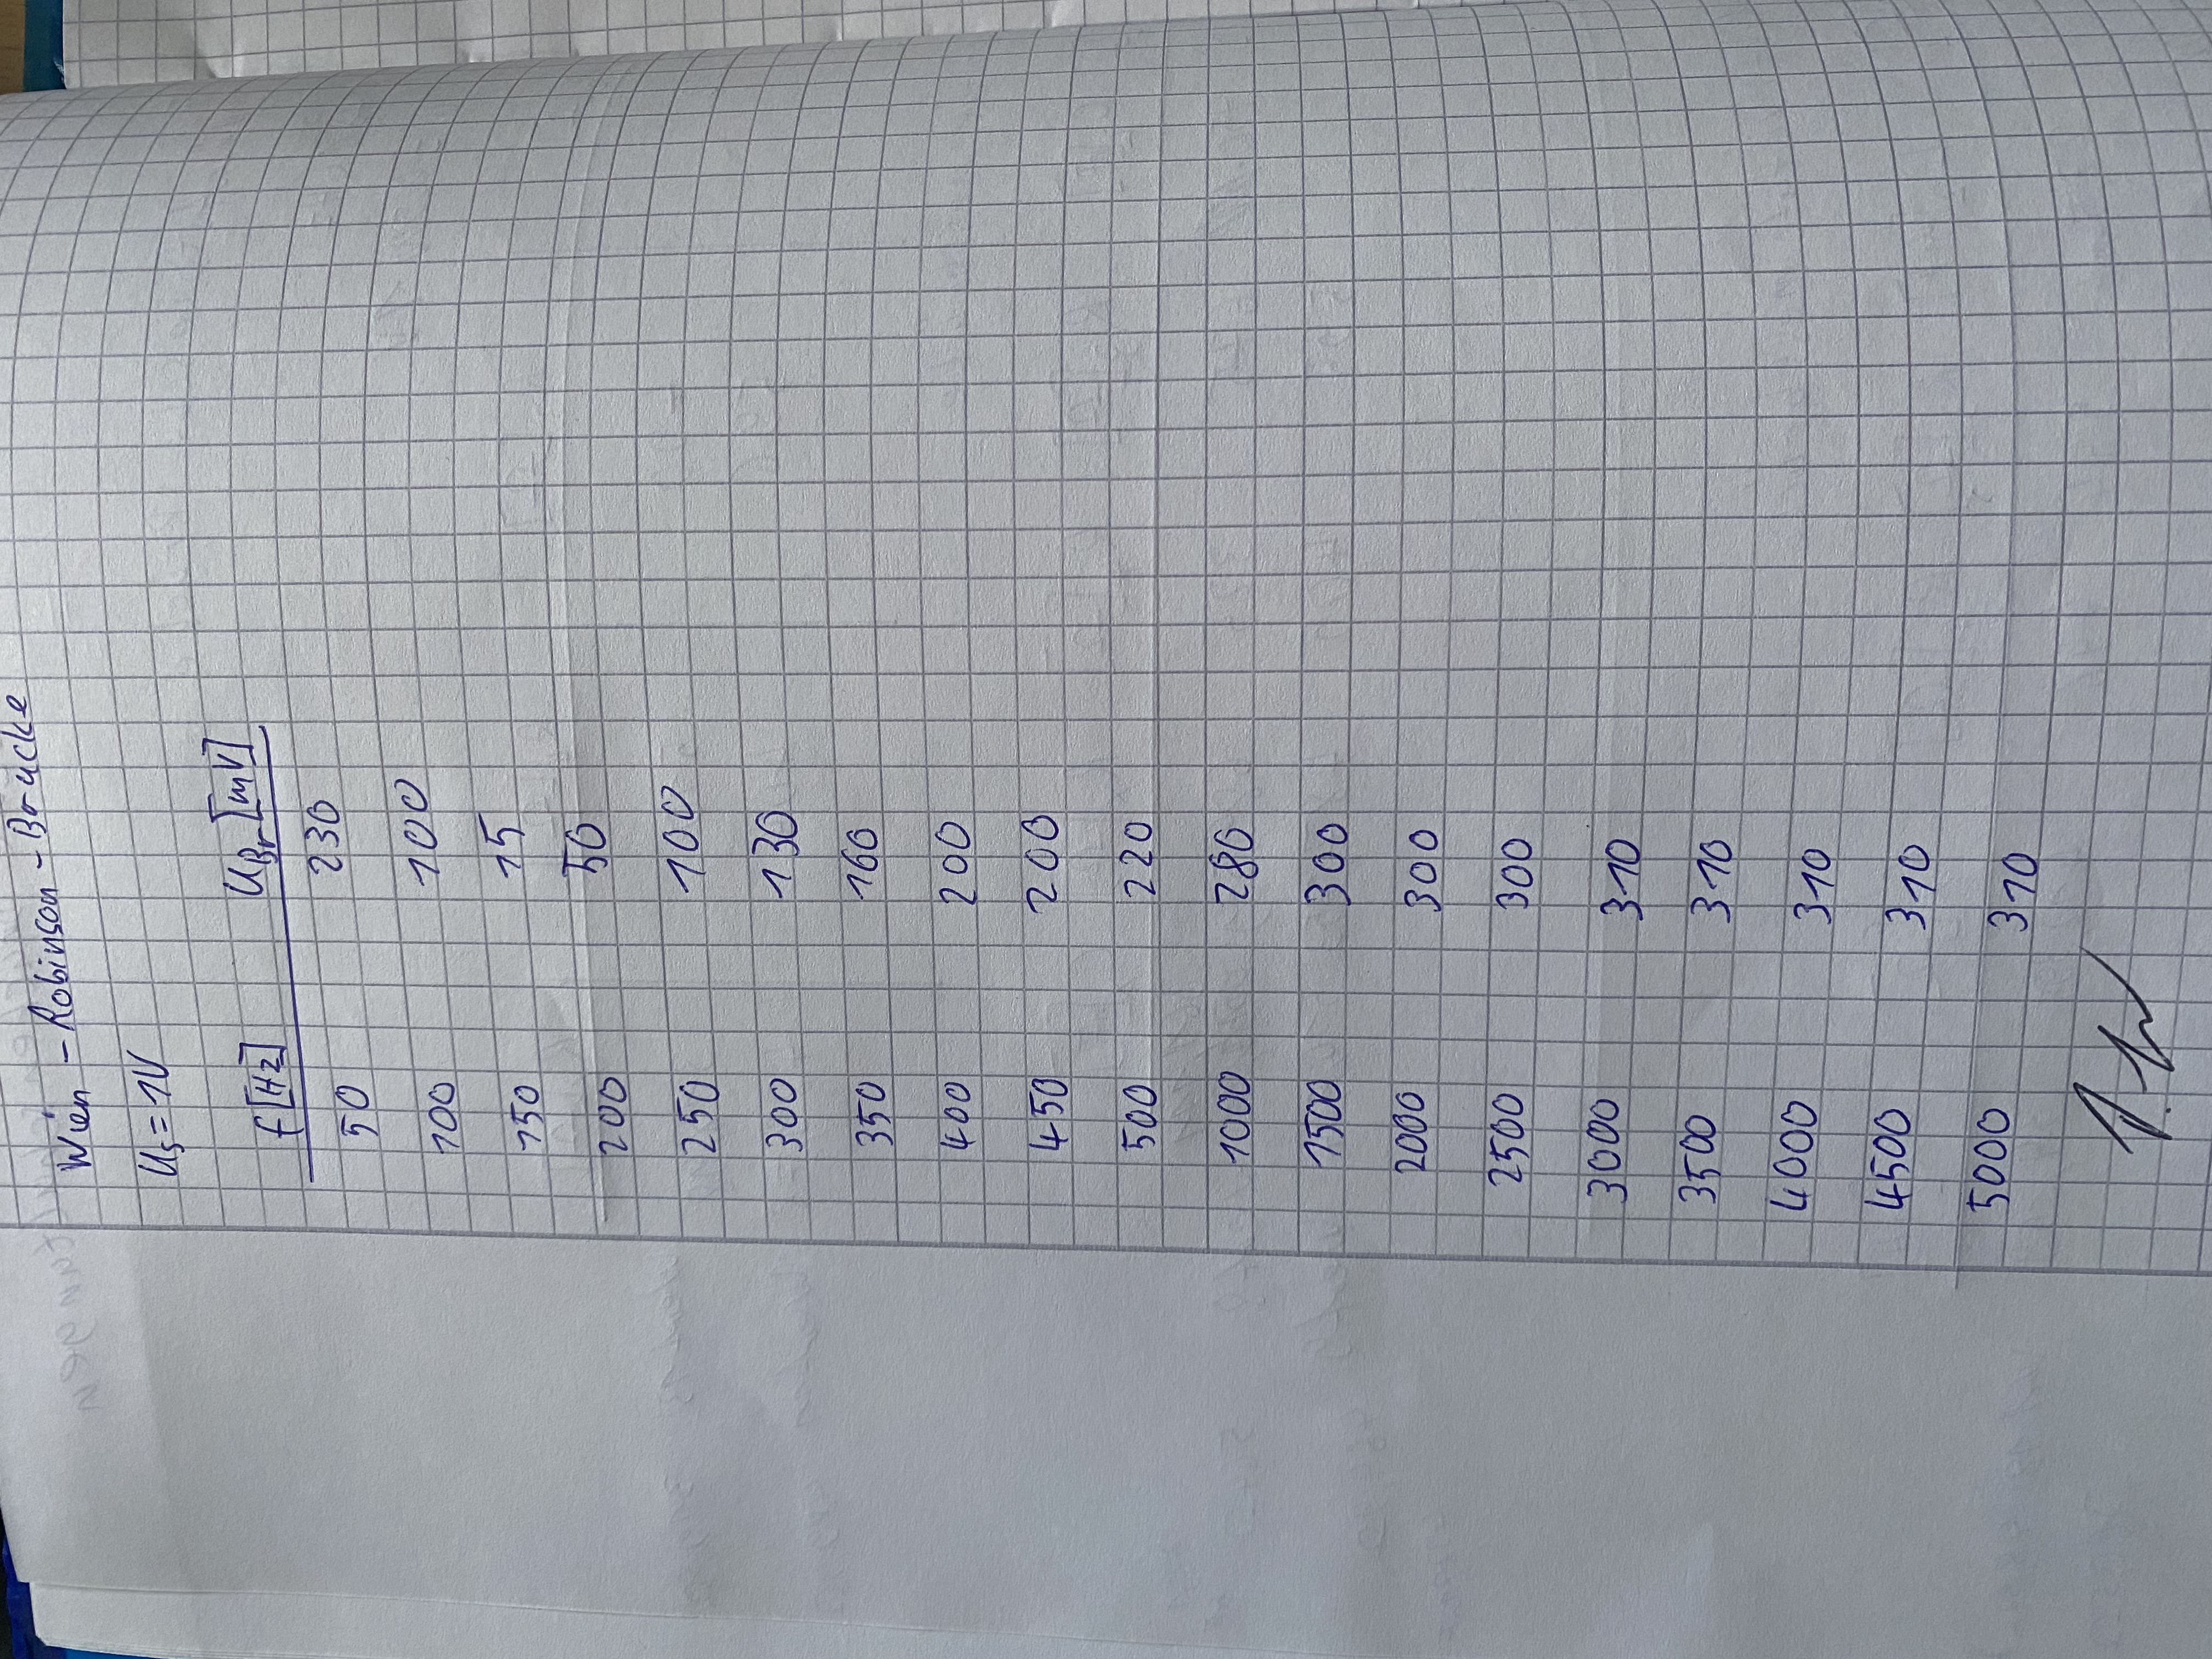
\includegraphics[scale=0.1, angle=270]{Bilder/mess2.jpg}
  
    \label{fig:mess2}
  \end{figure}